\section{Motivating Examples}
\label{sec:motivation}

% \dongsun{It is necessary to clarify ``code change'' and ``software changes''.
% Since our technique is not limited to source code changes, this would be
% carefully addressed.}

In the development course of software project, developers regularly commit
changes to project repositories. While some of those changes may simply be
cosmetic, a few others may be somehow influential not only inside and/or beyond
the repositories but also immediately and/or long after they are applied.
An influential software change can be recognized as such for various reasons, not
all of which are known while the change is being performed.


To motivate our study, we consider influential change 
examples identified from the Linux kernel project.
% The Linux kernel project hosts the development of the code which is at the heart
% of the Linux operating system, i.e., all code that run with kernel privileges,
% including device drivers and file systems.
Linux is an appropriate subject as several changes in the kernel have
been influential. These changes are already highlighted in the literature~\cite{Palix10Faults,padioleau08} as
their long-term impact started to be noticed.
In this section, we present four different examples of influential changes in
Linux kernel and their impact.


\subsection{Collateral Evolution}
% The notion of collateral evolutions was first introduced by Padioleau~{\em et
% al.}~\cite{padioleau06} to describe essential changes in OS evolution.
In the Linux kernel, since driver code, which makes up over 70\% of the source
code, is heavily dependent on the rest of the OS, any change in the interfaces
exported by the kernel and driver support libraries can trigger a large number
of adjustments in the dependent drivers~\cite{padioleau06}. 

Such adjustments,
known as collateral evolution, can unfortunately be challenging to implement
correctly. Starting with Linux 2.5.4, the USB library function {\em
usb\_submit\_urb} (which implements message passing) takes a second argument for
explicitly specifying the context (which was previously inferred in the
function definition). The argument can take one of three values: GFP\_KERNEL (no
constraints), GFP\_ATOMIC (blocking is not allowed), or GFP\_NOIO (blocking is
allowed but not I/O)). Developers using this USB library must then parse their
own code to understand which context it should be as in the example of Figure~\ref{listing:usb}.

This leads to bugs that keep occurring.
A study by Pallix {\em et al.}~\cite{Palix10Faults} has reported that, due to
the complexity of the conditions governing the choice of the new argument for
{\em usb\_submit\_urb}, 71 of the 158 calls to this function were initially
transformed incorrectly to use GFP\_KERNEL instead of GFP\_ATOMIC.


This change is interesting and constantly influential to a large portion of the
kernel, as its real impact could only be predicted if the analysis took into
account the semantics of the change. However, the extent of influences made by
the change is difficult to detect immediately after
the commit time since existing
techniques~\cite{ren_chianti:_2004,zhang_faulttracer:_2012,robillard_retrieving_2008,sherriff_empirical_2008}
focus only on the short-term impact.


\begin{figure}[!ht]
\centering
% before fix
{\parbox{\linewidth}{
\lstinputlisting[linewidth={\linewidth},frame=tb]{listing/kernel-before.tex}
}}%
\caption{Code patch for adaption to the new definition of {\em usb\_submit\_urb}.
    In this case, when the API function is called, locks are held, so the programmer must use
    GFP\_ATOMIC to avoid blocking. Its influence was propagated to most
    drivers using this library and mostly resulted in defects.}
\label{listing:usb}
\end{figure}
% ===========================================================================


\subsection{Feature Replacement}
\label{sec:motivation2}

In general, the number of entries in each fault category (e.g., {\em NULL} or {\em Lock})
decreases over
time in the Linux code base~\cite{Palix10Faults}.
In Linux 2.6, however, as illustrated in Figure~\ref{fig:lock_rise}, there are
some versions in which we can see a sudden rise in the number of faults.
This was the case of faults in the Lock\footnote{To avoid {\em Lock/LockIntr}
faults, release acquired locks, restore disable interrupts and do not double
acquire locks~\cite{Palix10Faults,Diagnosys}.
%     To avoid {\em Float} faults, do not use floating point in kernel.\\
% To avoid {\em Size} faults, allocate enough memory to hold the type for which
% you are allocating.
} 
category in Linux 2.6.16 due to a replacement of
functionality implementation.
In Linux 2.6.16, the functions {\em mutex\_lock} and {\em mutex\_unlock} were
introduced to replace mutex-like occurrences of the semaphore functions {\em
down} and {\em up}. The study of Palix {\em et al.} again revealed that 9 of the
11 Lock faults introduced in Linux  2.6.16 and 23 of the 25 Lock faults
introduced in Linux 2.6.17 were in the use of {\em mutex\_lock}.

If the replacement is identified earlier as an influential change to most of
kernel components (and other applications), it may prevent the defects from
recurring everywhere since the change is likely to be an API
change~\cite{linares-vasquez_api_2013,dig_how_2006}.
The developer who committed the new feature did not realize the influence and thus,
there was no early heads-up for other developers.

% \tb{Again, this can be detected if one could interpolate that a change that
% adds an API and removes another is actually a feature replacement}

\begin{figure}[h!]% \centering
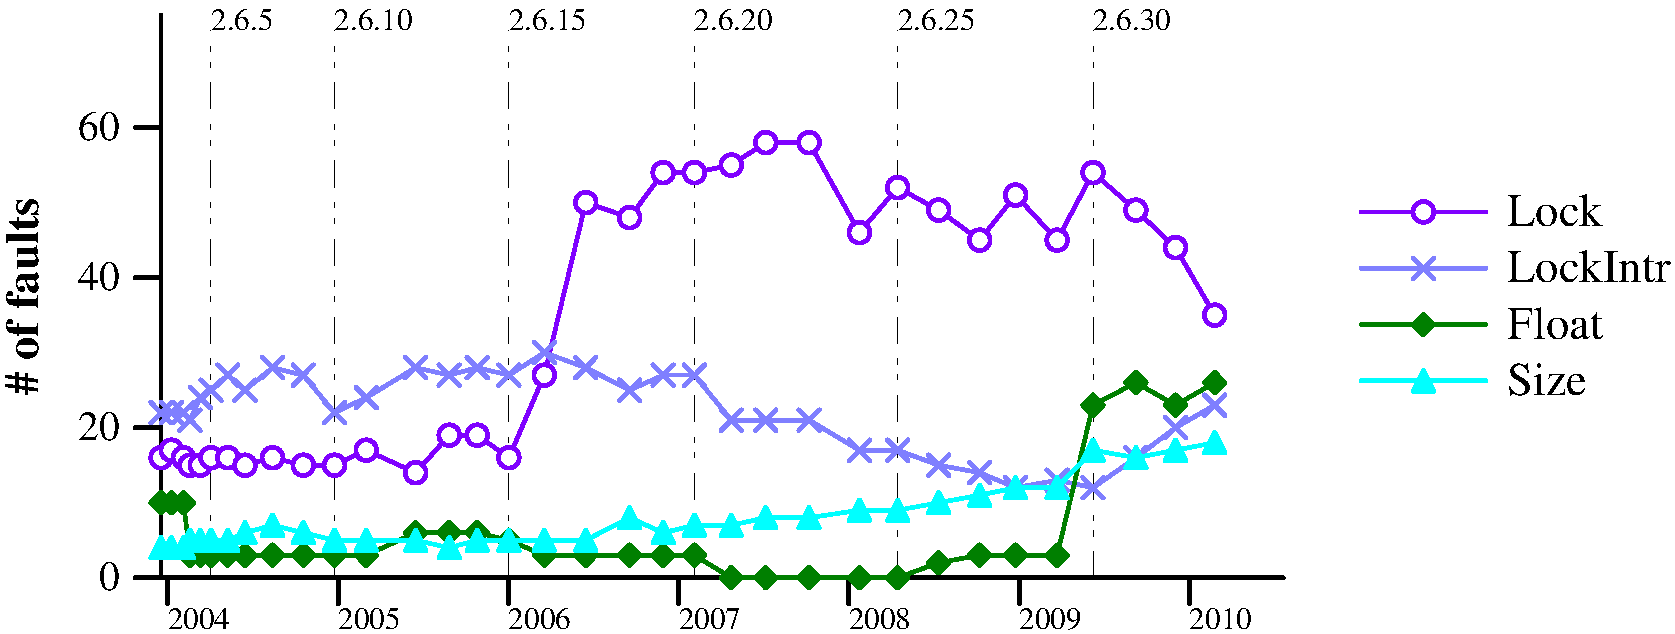
\includegraphics[width=\linewidth]{fig/feature-replacement} \caption{Evolution
of faults in Linux 2.6 kernel versions for {\em Lock}, {\em LockIntr}, {\em
Float} and {\em Size} fault categories~(see~\cite{Palix10Faults}). Faults
relevant to \emph{Lock} suddenly increased after Version 2.6.16 while other
types of faults gradually decreased. In the version, a feature for Lock was
replaced and it was influential to many of kernel functions.}
\label{fig:lock_rise}
\end{figure}


\subsection{Revolutionary Feature}

An obvious influential change may consist in providing an implementation of
a completely new feature, e.g., in the form of an API function.
In the Linux kernel repository, Git commit {\tt 9ac7849e} introduced device resource management
API for device drivers. Known as the {\em devm} functions, the API
provides memory management primitives for replacing {\em kzalloc} functions.
This code change is a typical example of influential change with a long-term impact.
As depicted in Figure~\ref{fig:devm}, this change has first gone unnoticed
before more and more people started using {\em devm} instead of {\em kzalloc}.
Had the developers recognized this change as highly influential, {\em devm} could have been adopted earlier and result in less bugs and better performance in driver code.


\begin{figure}[!h]%
    \centering
    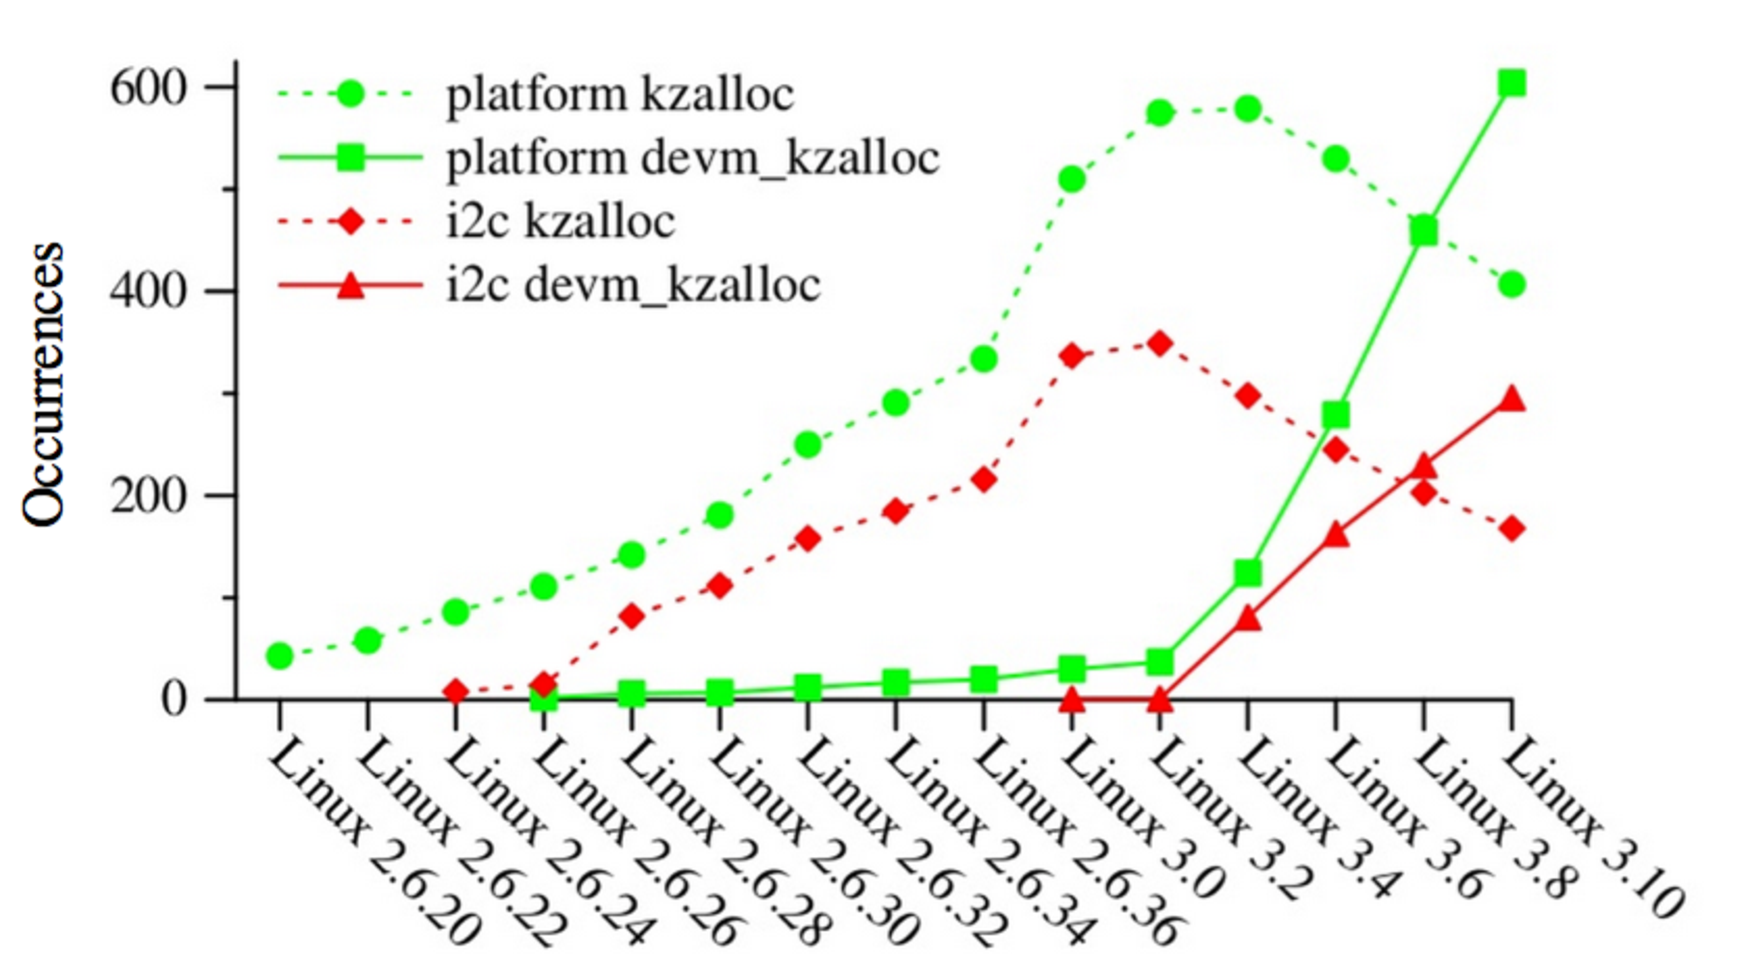
\includegraphics[width=0.8\linewidth]{fig/devm}
    \caption{Usage of memory allocation primitives in Linux kernel (See~\cite{recipes_devm}). {\em kzalloc} is the traditional API for memory allocation,
before managed memory ({\em devm}) was introduced in Linux.}
    \label{fig:devm}
\end{figure}


\subsection{Fixes of Controversial/Popular Issues}
Some issues in software projects can be abnormally discussed or commented longer than others.
Code changes that fix them will be influential for the project. The characteristics of a controversial/popular issue
 is that its resolution is of interest for a large number of developers, and it takes more time
to resolve them than the average time-to-fix delay. Thus, we consider that an issue report
which is commented on average more than other issues and is fixed very long after it
is opened, is about a controversial/popular issue. In Linux, Git commit {\tt bfd36103}
resolved Bug \#16691 which remained unresolved in the bug tracking system for 9 months
and was commented about 150 times.
